% !TeX encoding = UTF-8
% !TeX program = pdflatex
% !BIB program = biber

\documentclass[
        english,biblatex
    ]{lni}

% Standard packages
\usepackage{graphicx}
\usepackage{longtable}
\usepackage{booktabs}
\usepackage{array}
\usepackage{multirow}
\usepackage{wrapfig}
\usepackage{float}
\usepackage{colortbl}
\usepackage{pdflscape}
\usepackage{tabularx}
\usepackage{threeparttable}
\usepackage{threeparttablex}
\usepackage[normalem]{ulem}
\usepackage{makecell}

\usepackage{framed} % Needed for code blocks

\usepackage{color}
\usepackage{fancyvrb}
\newcommand{\VerbBar}{|}
\newcommand{\VERB}{\Verb[commandchars=\\\{\}]}
\DefineVerbatimEnvironment{Highlighting}{Verbatim}{commandchars=\\\{\}}
% Add ',fontsize=\small' for more characters per line
\usepackage{framed}
\definecolor{shadecolor}{RGB}{241,243,245}
\newenvironment{Shaded}{\begin{snugshade}}{\end{snugshade}}
\newcommand{\AlertTok}[1]{\textcolor[rgb]{0.68,0.00,0.00}{#1}}
\newcommand{\AnnotationTok}[1]{\textcolor[rgb]{0.37,0.37,0.37}{#1}}
\newcommand{\AttributeTok}[1]{\textcolor[rgb]{0.40,0.45,0.13}{#1}}
\newcommand{\BaseNTok}[1]{\textcolor[rgb]{0.68,0.00,0.00}{#1}}
\newcommand{\BuiltInTok}[1]{\textcolor[rgb]{0.00,0.23,0.31}{#1}}
\newcommand{\CharTok}[1]{\textcolor[rgb]{0.13,0.47,0.30}{#1}}
\newcommand{\CommentTok}[1]{\textcolor[rgb]{0.37,0.37,0.37}{#1}}
\newcommand{\CommentVarTok}[1]{\textcolor[rgb]{0.37,0.37,0.37}{\textit{#1}}}
\newcommand{\ConstantTok}[1]{\textcolor[rgb]{0.56,0.35,0.01}{#1}}
\newcommand{\ControlFlowTok}[1]{\textcolor[rgb]{0.00,0.23,0.31}{\textbf{#1}}}
\newcommand{\DataTypeTok}[1]{\textcolor[rgb]{0.68,0.00,0.00}{#1}}
\newcommand{\DecValTok}[1]{\textcolor[rgb]{0.68,0.00,0.00}{#1}}
\newcommand{\DocumentationTok}[1]{\textcolor[rgb]{0.37,0.37,0.37}{\textit{#1}}}
\newcommand{\ErrorTok}[1]{\textcolor[rgb]{0.68,0.00,0.00}{#1}}
\newcommand{\ExtensionTok}[1]{\textcolor[rgb]{0.00,0.23,0.31}{#1}}
\newcommand{\FloatTok}[1]{\textcolor[rgb]{0.68,0.00,0.00}{#1}}
\newcommand{\FunctionTok}[1]{\textcolor[rgb]{0.28,0.35,0.67}{#1}}
\newcommand{\ImportTok}[1]{\textcolor[rgb]{0.00,0.46,0.62}{#1}}
\newcommand{\InformationTok}[1]{\textcolor[rgb]{0.37,0.37,0.37}{#1}}
\newcommand{\KeywordTok}[1]{\textcolor[rgb]{0.00,0.23,0.31}{\textbf{#1}}}
\newcommand{\NormalTok}[1]{\textcolor[rgb]{0.00,0.23,0.31}{#1}}
\newcommand{\OperatorTok}[1]{\textcolor[rgb]{0.37,0.37,0.37}{#1}}
\newcommand{\OtherTok}[1]{\textcolor[rgb]{0.00,0.23,0.31}{#1}}
\newcommand{\PreprocessorTok}[1]{\textcolor[rgb]{0.68,0.00,0.00}{#1}}
\newcommand{\RegionMarkerTok}[1]{\textcolor[rgb]{0.00,0.23,0.31}{#1}}
\newcommand{\SpecialCharTok}[1]{\textcolor[rgb]{0.37,0.37,0.37}{#1}}
\newcommand{\SpecialStringTok}[1]{\textcolor[rgb]{0.13,0.47,0.30}{#1}}
\newcommand{\StringTok}[1]{\textcolor[rgb]{0.13,0.47,0.30}{#1}}
\newcommand{\VariableTok}[1]{\textcolor[rgb]{0.07,0.07,0.07}{#1}}
\newcommand{\VerbatimStringTok}[1]{\textcolor[rgb]{0.13,0.47,0.30}{#1}}
\newcommand{\WarningTok}[1]{\textcolor[rgb]{0.37,0.37,0.37}{\textit{#1}}}




\begin{document}

% Title
        \title[]{The difference between RSE and Data Science}
    
    
    \author[1,2]{Firstname1 Lastname1}{firstname1.lastname1@affiliation1.org}{0000-0000-0000-0000}
    \author[2]{Firstname2 Lastname2}{firstname2.lastname2@affiliation2.org}{0000-0000-0000-0000}
    \author[3]{Firstname3 Lastname3}{firstname3.lastname3@affiliation1.org}{0000-0000-0000-0000}
    \author[1]{Firstname4 Lastname4}{firstname4.lastname4@affiliation1.org}{0000-0000-0000-0000}%
    \affil[1]{Universität 1\\Abteilung\\Straße\\Postleitzahl Ort\\Land}
    \affil[2]{University 2 \\Department\\Address\\Country}
    \affil[3]{University 3\\Department\\Address\\Country}




    \maketitle

% Abstract
        \begin{abstract}
        Die LaTeX-Klasse \texttt{lni} setzt die Layout-Vorgaben für
        Beiträge in LNI Konferenzbänden um. Dieses Dokument beschreibt
        ihre Verwendung und ist ein Beispiel für die entsprechende
        Darstellung.
    \end{abstract}
    
% Keywords
        \begin{keywords}
        LNI Guidelines \and LaTeX Vorlage
    \end{keywords}
    
% Body
    \section{Verwendung}\label{verwendung}

    Die GI gibt unter http://www.gi-ev.de/LNI Vorgaben für die
    Formatierung von Dokumenten in der LNI Reihe.

    \section{Demonstrationen}\label{demos}

    \section{Demonstration der Einhaltung der
    Richtlinien}\label{lniconformance}

    \subsection{Literaturverzeichnis}\label{literaturverzeichnis}

    Beispielhafte Zitierungen: \textcite{Ez10}, \textcite{AB00}.

    \section{Abbildungen}\label{abbildungen}

    \begin{figure}

    \centering{

    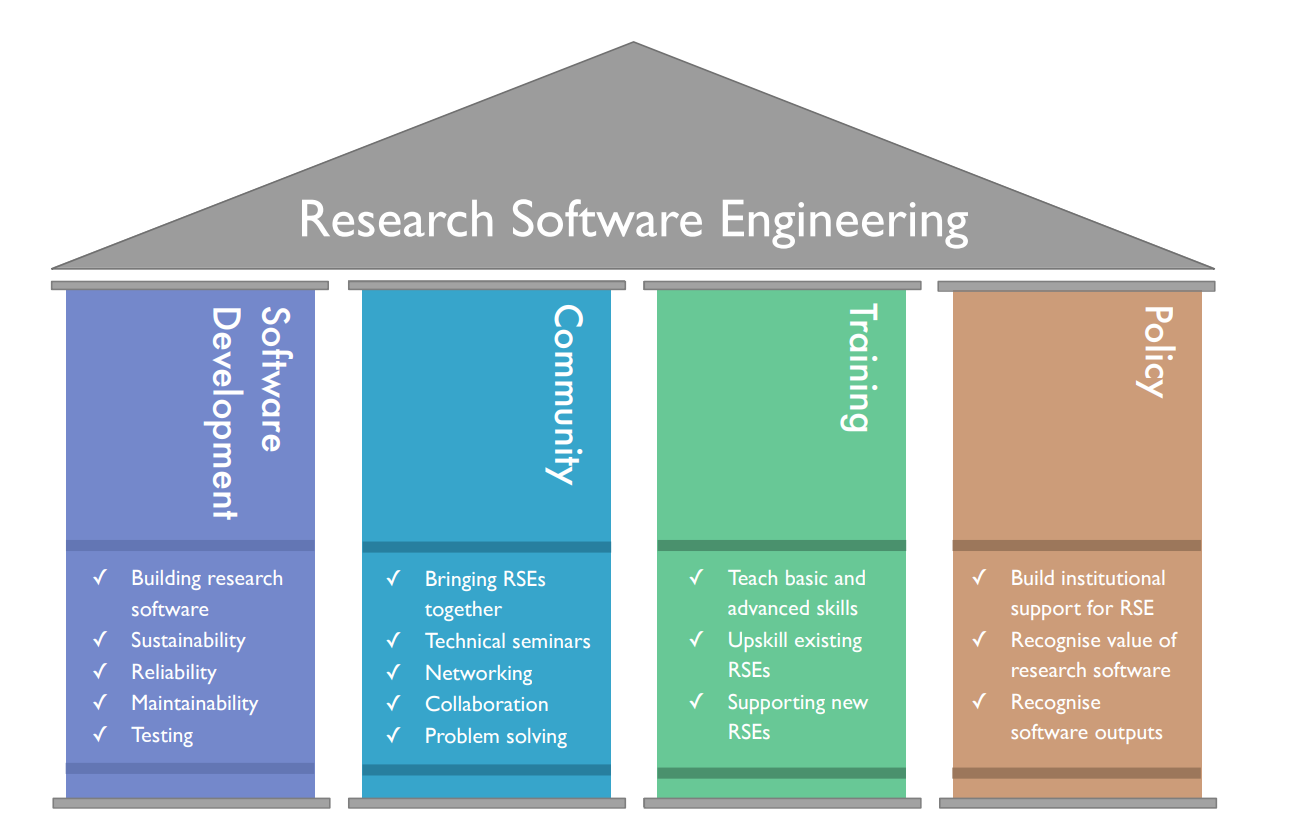
\includegraphics[width=0.8\linewidth,height=\textheight,keepaspectratio]{four_pillars_rse.png}

    }

    \caption{\label{fig-demo}Demographik}

    \end{figure}%

    \section{Tabellen}\label{tabellen}

    \begin{longtable}[]{@{}lll@{}}
    \caption{Die Überschriftsarten \{\#tab-demo\}}\tabularnewline
    \toprule\noalign{}
    Überschriftsebenen & Beispiel & Schriftgröße und -art \\
    \midrule\noalign{}
    \endfirsthead
    \toprule\noalign{}
    Überschriftsebenen & Beispiel & Schriftgröße und -art \\
    \midrule\noalign{}
    \endhead
    \bottomrule\noalign{}
    \endlastfoot
    Titel (linksbündig) & Der Titel \ldots{} & 14 pt, Fett \\
    Überschrift 1 & 1 Einleitung & 12 pt, Fett \\
    Überschrift 2 & 2.1 Titel & 10 pt, Fett \\
    \end{longtable}

    \section{Programmcode}\label{programmcode}

\begin{Shaded}
\begin{Highlighting}[]
\KeywordTok{public} \KeywordTok{class}\NormalTok{ Hello }\OperatorTok{\{}
    \KeywordTok{public} \DataTypeTok{static} \DataTypeTok{void} \FunctionTok{main} \OperatorTok{(}\BuiltInTok{String}\OperatorTok{[]}\NormalTok{ args}\OperatorTok{)} \OperatorTok{\{}
        \BuiltInTok{System}\OperatorTok{.}\FunctionTok{out}\OperatorTok{.}\FunctionTok{println}\OperatorTok{(}\StringTok{"Hello World!"}\OperatorTok{);}
    \OperatorTok{\}}
\OperatorTok{\}}
\end{Highlighting}
\end{Shaded}


% Bibliography
        \printbibliography
    
\end{document}
